\documentclass[11pt]{article}
\usepackage[scaled=0.92]{helvet}
\usepackage{geometry}
\geometry{letterpaper,tmargin=1in,bmargin=1in,lmargin=1in,rmargin=1in}
\usepackage[parfill]{parskip} % Activate to begin paragraphs with an empty line rather than an indent %\usepackage{graphicx}
\usepackage{amsmath,amssymb, mathrsfs, dsfont}
\usepackage{tabularx}
\usepackage[font=footnotesize,labelfont=bf]{caption}
\usepackage{graphicx}
\usepackage{xcolor}
%\usepackage[linkbordercolor ={1 1 1} ]{hyperref}
%\usepackage[sf]{titlesec}
\usepackage{natbib}
\usepackage{../../Tianpei_Report}
%\usepackage{appendix}
%\usepackage{algorithm}
%\usepackage{algorithmic}

%\renewcommand{\algorithmicrequire}{\textbf{Input:}}
%\renewcommand{\algorithmicensure}{\textbf{Output:}}



\begin{document}
\title{Lecture 1: Causal Inference}
\author{ Tianpei Xie}
\date{Sep. 5th., 2022 }
\maketitle
\tableofcontents
\newpage
\allowdisplaybreaks
\section{Motivation: association does not imply causation}
\begin{itemize}
\item The aim of \emph{\textbf{standard statistical analysis}}, typified by regression, estimation, and hypothesis testing techniques, is to assess parameters of a \textbf{distribution} from samples drawn of that distribution.

\item  \emph{\textbf{Causal analysis}}  aim at inferring not only beliefs or probabilities under static conditions, but also the \emph{\textbf{dynamics}} of beliefs under \emph{\textbf{changing conditions}}, for example, changes induced by treatments or external interventions.

\item there is nothing in a distribution function to tell us how that distribution would differ \emph{\textbf{if external conditions were to change}} -- say from \underline{\textbf{\emph{observational}}} to \underline{\textbf{\emph{experimental}}} setup -- because the laws of probability theory do not dictate how one property
of a distribution ought to change when another property is modified. This information must be provided by \emph{\textbf{causal assumptions}} which identify relationships
that remain invariant when external conditions change. \citep{pearl2009causal}

\item \emph{\textbf{Association does not imply causation}}: one cannot \emph{substantiate} \textbf{causal} claims from \textbf{\emph{associations}} alone, even at the population level -- behind every causal conclusion there must lie some \emph{causal assumption} that is \textbf{not testable in observational studies}. \citep{pearl2009causal}

\item An \emph{\textbf{associational concept}} is any relationship that can be defined in terms of a \textbf{joint distribution} of observed variables, and a \emph{\textbf{causal concept}} is any relationship that \emph{\textbf{cannot} be defined} from the distribution alone.
\begin{itemize}
\item Examples of \underline{\emph{associational concepts}} are: \emph{correlation}, \emph{regression}, \emph{dependence}, \emph{conditional independence}, \emph{likelihood}, \emph{collapsibility}, propensity score, \emph{risk ratio}, \emph{odds ratio}, \emph{marginalization}, \emph{conditionalization}, “controlling for.”
\item Examples of \underline{\emph{causal concepts}} are: \emph{\textbf{randomization}}, influence, effect, \emph{\textbf{confounding}}, “holding constant,” disturbance,
\emph{\textbf{spurious correlation}}, faithfulness/stability, instrumental variables, \emph{\textbf{intervention}}, explanation, \emph{\textbf{attribution}}, and so on.
\end{itemize}
\end{itemize}

\subsection{Simpson's Paradox}
\begin{figure}
\begin{minipage}[t]{1\linewidth}
  \centering
  \centerline{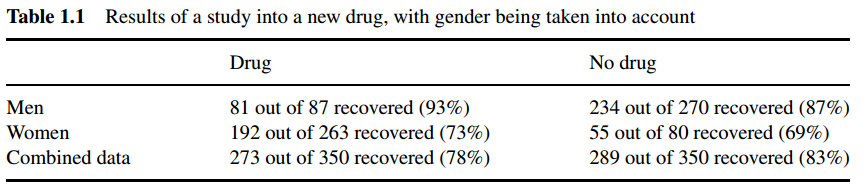
\includegraphics[scale = 0.5]{simpson_paradox.png}}
\end{minipage}
\caption{\footnotesize{\textbf{The example for Simpson paradox. The drug ha positive impact on each gender but not in total population. \citep{glymour2016causal}}}}
\label{fig: simpson_paradox}
\end{figure}
\begin{itemize}
\item \textbf{Simpson's Paradox}  refers to the existence of data in which a \emph{statistical association} that holds for an \emph{\textbf{entire population}} is \textbf{reversed} in \emph{\textbf{every subpopulation}}.

Figure \ref{fig: simpson_paradox} shows an example for a drug test. The first row shows the outcome for male patients; the second row shows the outcome for
female patients; and the third row shows the outcome for all patients, regardless of gender. In male patients, drug takers had a better recovery rate than those who went without the drug ($93\%$ vs $87\%$). In female patients, again, those who took the drug had a better recovery rate than nontakers ($73\%$ vs $69\%$). However, in the combined population, those who did not take the drug had a better recovery rate than those who did ($83\%$ vs $78\%$).

The data seem to say that if we know the patient’s gender -- male or female -- we can prescribe the drug, but if the gender is unknown we should not! 

\begin{figure}
\begin{minipage}[t]{0.5\linewidth}
  \centering
  \centerline{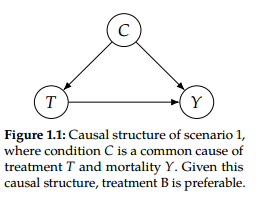
\includegraphics[scale = 0.7]{simpson_paradox_causal_1.png}}
\end{minipage}
\begin{minipage}[t]{0.5\linewidth}
  \centering
  \centerline{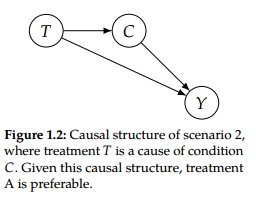
\includegraphics[scale = 0.7]{simpson_paradox_causal_2.png}}
\end{minipage}
\caption{\footnotesize{\textbf{The causal dependency of external condition $C$ to precscription of treatment $T$ and its outcome $Y$. \citep{neal2020introduction}}}}
\label{fig: simpson_paradox_causal}
\end{figure}
\item \emph{\textbf{Causality}} is essential to solve Simpson’s paradox. The solution depends on the causal structure. 
\begin{itemize}
\item[\textbf{Scenario 1:}] If there is an external condition $C$ that \textbf{both causes the treatment} $T$ of drug, \textbf{and affects} the recovery $Y$. Like Figure \ref{fig: simpson_paradox_causal} left. For instance, in the table in \ref{fig: simpson_paradox}, a portion of element in the drug will negatively affect women's recovery more than men. Also we see that women are significantly more likely to take the drug than men are. So, the reason the drug appears to be harmful
overall is that, if we select a drug user at random, that person is more likely to be a woman and hence less likely to recover than a random person who does not take the drug. Condition $C$ is "being women".

\item[\textbf{Scenario 2:}] If the \emph{\textbf{prescription}} of treatment $T$ is a \emph{\textbf{cause}} of condition $C$, and both $T$ and $C$ affect the outcome $Y$. Like Figure \ref{fig: simpson_paradox_causal} right. For instance,  presciption of the drug requires a long delay before the treatment and the long delay negatively affects the recovery.  
\end{itemize}

\item The key assumption missing in Simpson's paradox is that the \emph{treatment cannot not affect sex}. In other words, it assumes that \emph{the \textbf{partition variable} itself cannot be a factor determing the outcome}. If it could, there would be no paradox since the causal strcuture will explain the result. 
\end{itemize}

\subsection{Main Themes}
\begin{itemize}
\item \textbf{Statistical vs. Causal}: Even with an infinite amount of data, \textbf{we sometimes cannot compute some causal quantities}. In contrast, much of
statistics is about \emph{addressing uncertainty} in finite samples. Association, a statistical concept, is not causation. There is more work to be done in causal inference, even after starting with infinite data. This is the \textbf{main distinction} motivating \textbf{\emph{causal inference}}. 

\item \textbf{Identification vs. Estimation}: \emph{Identification} of causal effects is \textbf{unique} and challenging  in causal inference. However, causal inference also shares \emph{estimation} with traditional statistics and machine learning.

\item \textbf{Interventional vs. Observational}: If we can \textbf{intervene/experiment}, identification of causal effects is relatively easy. We can simply measure the effect after we take that action. \emph{Observational} data is where it gets more complicated because \textbf{confounding} is almost always introduced into the data.

\item \textbf{Assumptions}: There will be a large focus on what assumptions we are using to get the results that we get. Each assumption will have its own
box to help make it difficult to not notice. \textbf{Clear assumptions} should make it easy to see where critiques of a given causal analysis or causal model will be. The hope is that presenting assumptions clearly will lead to more lucid discussions about causality.
\end{itemize}

\section{Potential Outcomes}
\subsection{Potential Outcomes and Individual Treatment Effects}
We will use $T \in  \set{0, 1}$ to denote the random variable for treatment,  $Y$ to denote the random variable for the outcome of interest and $X$ to denote covariates. 
\begin{itemize}
\item The \emph{\textbf{potential outcome}} $Y(t)$ denotes what your outcome \textbf{would be}, if you \textbf{were} to take treatment $T=t$. A potential outcome $Y(t)$ is distinct from the \emph{\textbf{observed}} outcome $Y$ in that \underline{\emph{not all potential outcomes are observed}}. Rather all potential outcomes can potentially be observed. The one that is \emph{actually observed} depends on the value that the treatment $T$ takes on.

\item \textbf{Before} treatment, any outcome is \emph{potential outcome}. \textbf{After} treatment, one outcome is \emph{observed outcome} (i.e. $(Y(1)\, |\, T=1)$ and $(Y(0)\, |\, T=0)$) and the rest are \emph{\textbf{counterfactual outcomes}} (i.e. $(Y(1)\, |\, T=0)$ and $(Y(0)\, |\, T=1)$).

\item Although only one of the outcome can be observed for one individual, there are many people in the population. We will denote the treatment, covariates, and
outcome of the $i$-th individual using $T_i$,  $X_i$, and $Y_i$. Then, we can define the \underline{\emph{\textbf{individual treatment effect (ITE)}}} \citep{neal2020introduction} for individual $i$:
\begin{align}
\tau_i &= Y_i(1) - Y_i(0) \label{eqn: ITE}
\end{align} Whenever there is more than one individual in a population, $Y(t)$ is a random variable because different individuals will have different potential
outcomes. In contrast, $Y_i(t)$  is usually treated as \textbf{non-random} because the subscript $i$ means that we are conditioning on so much individualized (and context-specific) information, that we restrict our focus to a single individual (in a specific context) whose potential outcomes are deterministic.

\item ITEs are some of the main quantities that we care about in causal inference.
\end{itemize}

\subsection{The Fundamental Problem of Causal Inference}
It is impossible to observe \textbf{all potential outcomes} for a given individual in \eqref{eqn: ITE}. This is known as \underline{\emph{\textbf{the fundamental problem of causal inference}}}. It is fundamental because if we cannot observe both $Y_i(1)$ and $Y_i(0)$, then we cannot observe the causal effect $Y_i(1) - Y_i(0)$. This problem is \textbf{unique} to causal inference because, in causal inference, we care about making causal claims, which are defined in terms of potential outcomes. 

The potential outcomes that you \emph{do not (and cannot) observe} are known as \underline{\emph{\textbf{counterfactuals}}} because they are counter to fact (reality). In contrast, the potential outcome that is \textbf{observed} is sometimes referred to as a \emph{factual}. 

\subsection{Average Treatment Effects and Causal Assumptions}
\begin{figure}
\begin{minipage}[t]{1\linewidth}
  \centering
  \centerline{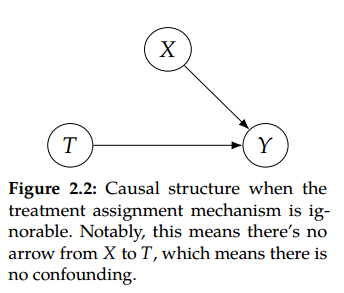
\includegraphics[scale = 0.5]{ignorability.png}}
\end{minipage}
\caption{\footnotesize{\textbf{The Causal structure when the
treatment assignment mechanism is ignorable.  \citep{neal2020introduction}}}}
\label{fig: ignorability}
\end{figure}

\begin{itemize}
\item Given a populuation, we can compute the \underline{\emph{\textbf{average treatment effect (ATE)}}}, or, \emph{average causal effect (ACE)} \citep{neal2020introduction}  by taking an average over the ITEs:
\begin{align}
\tau &:=  \E{}{Y_i(1) - Y_i(0)} =  \E{}{Y(1)} -\E{}{Y(0)} \label{eqn: ATE}
\end{align} where the average is over the individuals $i$ if $Y_i(t)$ is deterministic. If $Y_i(t)$ is random, the average is also over any other randomness.

\item A natural quantity that comes to mind is the \emph{\textbf{associational difference}}:
\begin{align}
\delta &:= \E{}{Y| T = 1} - \E{}{Y| T = 0} \label{eqn: associational_difference}
\end{align} Note that in general,  \eqref{eqn: associational_difference} is not equal to \eqref{eqn: ATE} since $\E{}{Y| T = 1}$ is the expectation of outcome on a \underline{\emph{\textbf{sub-population}}} with treatment $T=1$ while $ \E{}{Y(1)}$ is the expectation of outcome if the treatment \emph{\textbf{on the \underline{whole population} was}} $T=1$.  The former is an associational quality and association does not equal to causation. $\delta$ is comparing \emph{\textbf{two populations}} of people while $\tau$ is comparing what would happen if the \textbf{same people} were given different treatments.
\end{itemize}

\subsubsection{Ignorability and Exchangeability}
\begin{itemize}
\item Although one of potential outcomes are not observed, we can choose to ignore them and compute $ \E{}{Y(1)}$ by taking average over observed outcomes. Assuming \textbf{ignorability} is like \textbf{ignoring} how people ended up \textbf{selecting} the treatment they selected and just \textbf{assuming they were randomly assigned} their treatment. Formally, we have
\begin{assumption} (\textbf{Ignorability / Exchangeability}) \citep{neal2020introduction}
\begin{align}
(Y(1), Y(0)) \indep T  \label{eqn: Ignorability}
\end{align}
\end{assumption}The ignorability is a key assumption to causal inference because it allows us to reduce the ATE to the associational difference, i.e. $\tau = \E{}{Y(1)} -\E{}{Y(0)} = \E{}{Y| T = 1} - \E{}{Y| T = 0} = \delta$. Under this assumption, there is no confounding factor that allows the treatment selection have effects on the outcome after it is selected (i.e. \emph{\textbf{no unmeasured confounders}}). Figure \ref{fig: ignorability} shows the causal structure behind exhangeablility. 

\item Remember $Y(0)$ and $Y(1)$ are both random variables themselves even if the treatment $T=0,1$ is fixed. $P(Y(0)\,|\,T=1)$ answers the \emph{\textbf{counterfactual question}} "what potential outcome \emph{would be} if I \emph{did not} select treatment ?"

\item Another perspective on this assumption is that of \emph{\textbf{exchangeability}}. This assumption means $\E{}{Y(1)\,| T = 0}=\E{}{Y(1)\,| T = 1}$
and $\E{}{Y(0)\,| T = 0}=\E{}{Y(0)\,| T = 1}$ , respectively. Then, this implies $\E{}{Y(1)\,| T = t}=\E{}{Y(1)}$  and $\E{}{Y(0)\,| T = t}=\E{}{Y(0)}$ for all $t$. Exchangeability means that the \textbf{\emph{treatment groups are exchangeable}} in the sense that if they were \textbf{swapped}, the new treatment group would observe the \textbf{same outcomes} as the old treatment group, and the new control group would observe the same outcomes as the old control group. In this sense, our choice of test subjects are nothing special for treatement vs. control. 

An important \textbf{intuition} to have about exchangeability is that it guarantees that the \textbf{\emph{treatment groups are \underline{comparable}}}. In other words, the control and treatment groups are the same in all relevant aspects other than the treatment.  This intuition is what underlies the concept of "\textbf{controlling} for" or "adjusting for" variables.

\item 
\begin{definition}(\textbf{\emph{Identifiability}}) \citep{neal2020introduction}\\
 A \emph{causal} quantity (e.g. $\E{}{Y(t)}$) is \emph{\textbf{identifiable}} if we can compute it from a purely statistical quantity (e.g.  $\E{}{Y\,| T = t}$).
\end{definition} To identify a causal effect is to reduce a causal expression to a purely statistical expression. It means to reduce the potential outcomes to conditioning and expectation.

\item \textbf{\emph{Randomized experiments}} are the key for ignorability assumption to hold. With \emph{randomization}, we can safely assume that both observed and unobserved covariates are \emph{\textbf{balanced}}. 

\item Under randomized experiments, the \emph{\textbf{expectation}} of ITE can be estimated by the \emph{\textbf{average outcomes}} from both control and treatment groups. Moreover, the expected outcome given only one treatment $T=1$ for entire population $\E{}{Y(1)}$ can be estimated by the average outcome from the treatment group. Same for $T=0$.
\end{itemize}

\subsubsection{Conditional Exchangeability and Unconfoundedness}
\begin{figure}
\begin{minipage}[t]{0.5\linewidth}
  \centering
  \centerline{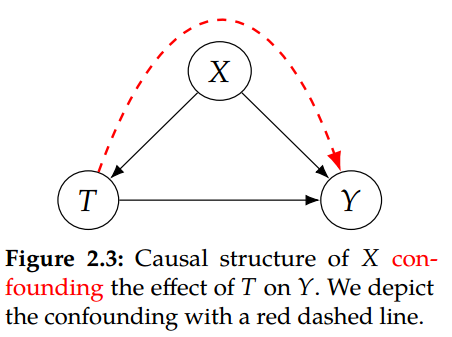
\includegraphics[scale = 0.4]{cond_exch_1.png}}
\end{minipage}
\begin{minipage}[t]{0.5\linewidth}
  \centering
  \centerline{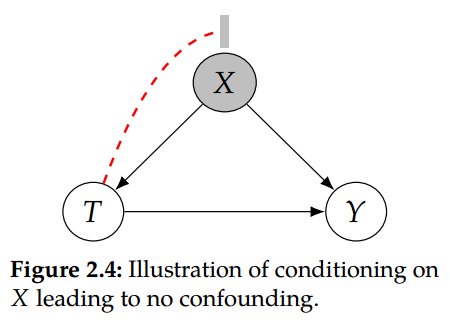
\includegraphics[scale = 0.4]{cond_exch_2.png}}
\end{minipage}
\caption{\footnotesize{\textbf{Illustration of conditioning on $X$ leading to no confounding. \citep{neal2020introduction}}}}
\label{fig: cond_exch}
\end{figure}

\begin{itemize}
\item There is no reason to expect that the groups are the same in all relevant variables other than the treatment. However, if we \textbf{control} for relevant variables by conditioning, then maybe the subgroups will be exchangeable. 
\begin{assumption} (\textbf{Conditional Exchangeability / Unconfoundedness}) \citep{neal2020introduction}
\begin{align}
(Y(1), Y(0)) \indep T \;|\; X \label{eqn: conditional_exchangeablity}
\end{align} 
\end{assumption} The idea is that although the treatment and potential outcomes may be unconditionally associated (due to confounding), \textbf{\emph{within levels of $X$}}, they are not associated. In other words, there is no confounding within levels of $X$ because controlling for $X$ has made the treatment groups comparable (i.e. randomly assigned). Figure \ref{fig: cond_exch} illustrate conditioning on $X$ the treatement and potential outcomes are independent.

\item \textbf{Conditional exchangeability is the main assumption necessary for causal inference}. Armed with this assumption, we can identify the causal effect
within levels of $X$, just like we did with (unconditional) exchangeability
\begin{align}
 \E{}{Y_i(1) - Y_i(0) | X} &=  \E{}{Y_i(1) \,|\,X } -\E{}{Y_i(0) \,|\, X} \nonumber\\
 &=  \E{}{Y \,|T=1,\,X } -\E{}{Y \,|T=0, \, X} \label{eqn: cond_ATE} \\
\tau= \E{}{Y_i(1) - Y_i(0)}&=\E{X}{ \E{}{Y_i(1) - Y_i(0)}|X} \nonumber\\
 &= \E{X}{ \E{}{Y \,|T=1,\,X }} - \E{X}{\E{}{Y \,|T=0, \, X}} \label{eqn: ATE_2} 
\end{align}

%\item For conditional exchangeability to hold, we need to control all observed covariates to be the same with only treatment assignments differ.  

\item \begin{theorem}(\textbf{Adjustment Formula})  \citep{neal2020introduction}\\
Given the assumptions of \textbf{unconfoundedness}, \textbf{positivity}, \textbf{consistency}, and \textbf{no interference}, we can identify the average treatment effect:
\begin{align*}
\tau= \E{}{Y(1) - Y(0)} &= \E{X}{ \E{}{Y \,|T=1,\,X }- \E{}{Y \,|T=0, \, X}}  
\end{align*}
\end{theorem}

\item The conditioning process $(\E{}{Y \,|T=1,\,X }- \E{}{Y \,|T=0, \, X})$ in \eqref{eqn: ATE_2} is called \textbf{\emph{stratification}}, i.e. we focus our estimation of treatment effects within each stratum $X=x$. The process of stratification and averaging is called  \emph{\textbf{standarization}}.
\end{itemize}

\subsubsection{Positivity/Overlap and Extrapolation}
\begin{itemize}
\item \emph{\textbf{Positivity}} is the condition that all subgroups of the data with different covariates have some probability of receiving \emph{\textbf{any value of treatment}}. Formally, we define positivity for binary treatment as follows
\begin{assumption} (\textbf{Positivity / Overlap / Common Support})  \citep{neal2020introduction}\\
For all values of covariates $x$ present in the population of interest (i.e. $x$ such that $P(X = x) > 0$),
\begin{align}
0 < P(T=1 | X = x) < 1 \label{eqn: positive}
\end{align}
\end{assumption} This assumption make sure for all choice of $X=x$, the condition on both $T=1$ and $X=x$ is well defined. 

\item If we have a positivity violation, that means that within some subgroup of the data, everyone always receives treatment or everyone always receives the control. It wouldn’t make sense to be able to estimate a causal effect of treatment vs. control in that subgroup since we see only treatment or only control. We never see the alternative in that subgroup.

\item Another name for positivity is \emph{\textbf{overlap}}. The intuition for this name is that we want the covariate distribution of the treatment group to overlap
with the covariate distribution of the control group. 

\item There is a \emph{\textbf{Positivity-Unconfoundedness Tradeoff}}: Conditioning on more covariates could lead to a higher chance of satisfying unconfoundedness. But it can lead to a higher chance of violating positivity. 

\item Violations of the positivity assumption can actually lead to demanding too much from models and getting very bad behavior in return. Note that the estimate $ \E{}{Y \,|T=t, \, X=x}$ requires all possible input pairs $(1, x)$ and $(0,x)$. These models will be forced
to extrapolate in regions (using their parametric assumptions) where $P(T=1, X = x) = 0$ and regions where $P(T=0, X = x) = 0$. 
\end{itemize}
\subsubsection{No interference, Consistency, and SUTVA}
\begin{itemize}
\item \textbf{\emph{No interference}} means that my outcome is unaffected by anyone else’s treatment. Rather, my outcome is only a function of my own treatment.
\begin{assumption}(\textbf{No Interference}) \citep{neal2020introduction}\\
\begin{align}
Y_{i}(t_1, \ldots, t_i, \ldots, t_n) &= Y_{i}(t_i) \label{eqn: no_interference}
\end{align}
\end{assumption}

\item \textbf{\emph{Consistency}} is the assumption that the outcome we \textbf{observe} $Y$ is actually the \textbf{potential outcome} under the \textbf{observed treatment} $T$.
\begin{assumption}(\textbf{Consistency}) \citep{neal2020introduction}\\
If the treatment is $T$, then the observed outcome $Y$ is the potential outcome under treatment $T$. Formally,
\begin{align}
T=t &\Rightarrow Y = Y(t) \label{eqn: consistency}
\end{align}
We could write this equivalently as follow:
\begin{align}
Y = Y(T) \label{eqn: consistency2}
\end{align}
\end{assumption} Note that $T$ is different from $t$, and $Y(T)$ is different from $Y(t)$.  $T$ is a
random variable that corresponds to the \textbf{observed treatment}, whereas $t$ is a specific value of treatment. Similarly, $Y(t)$ is the potential outcome for
some specific value of treatment, whereas $Y(T)$ is the potential outcome for the \emph{actual} value of treatment that we \textbf{observe}.

\item It may be confusing but the \textbf{potential outcome $Y(t)$ is a random variable itself due to intervention $T=t$}, and it is conceptually different from the random variable $Y$. Only via the consistency assumption \eqref{eqn: consistency} these two variables are connected.


\item By consistency assumption, we have
\begin{align*}
  \E{}{Y(1)\,| T = 1} - \E{}{Y(0)\,| T = 0} &= \E{}{Y| T = 1} - \E{}{Y| T = 0}
\end{align*} 

\item \textbf{\emph{Stable unit-treatment value assumption (SUTVA)}} is satisfied if unit (individual) $i$'s outcome is simply a \textbf{function} of unit $i$'s treatment. Therefore, SUTVA is a combination of consistency and no interference (and also \emph{\textbf{deterministic}} potential outcomes). 
\end{itemize}
\begin{figure}
\begin{minipage}[t]{1\linewidth}
  \centering
  \centerline{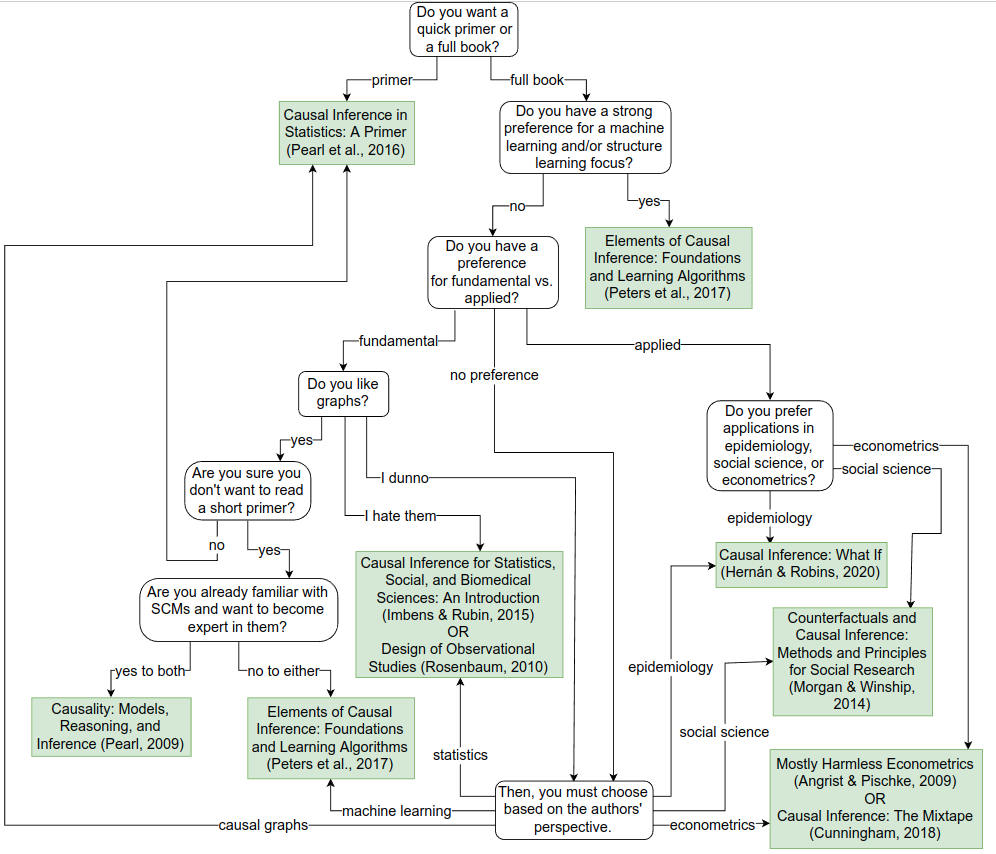
\includegraphics[scale = 0.42]{books_flowchart.png}}
\end{minipage}
\caption{\footnotesize{\textbf{Books for different areas in causal inference and analysis  \citep{neal2020introduction}}}}
\label{fig: books_flowchart}
\end{figure}
\section{Structural Causal Models}
An alternative viewpoint to the \underline{\emph{\textbf{Potential Outcome (PO) model}}} \citep{imbens2015causal, rosenbaum2017observation} is the \underline{\emph{\textbf{Structural Causal Model}}} \textbf{(SCM)} \citep{pearl2000causal, pearl2009causal, glymour2016causal}. This model as well as \textbf{Causal Bayesian Networks} \citep{pearl2000causal, pearl2009causal} are ways of describing the relevant features of the world and how they interact with each other based on  \textbf{Directed Acyclic Graphs (DAG)}.
\begin{itemize}
\item \begin{definition} (\emph{\textbf{Structural Causal Model (SCM)}})\\
 A \emph{structural causal model} is a tuple of the following sets:
 \begin{enumerate}
 \item a set of \emph{internal variables} $\mb{V}$ called \underline{\textbf{\emph{endogenous}}} variables;
 \item a set of \emph{external variables} $\mb{U}$ called  \underline{\textbf{\emph{exogenous}}} variables;
 \item and \underline{a set of \emph{\textbf{functions}} $\mb{F}$} that determine the values of the the variables in $\mb{V}$ based on the values of the variables in $\mb{U}$.
\end{enumerate} 
\end{definition}

\item The exogenous variables in $\mb{U}$ are \textbf{external} to the model; we choose not to explain how they are caused.  \emph{Exogenous variables \textbf{cannot be descendants} of any other variables}, and in particular, cannot be a descendant of an endogenous variable; they have \textbf{no ancestors} and are represented as \textbf{root nodes} in graphs.

Every endogenous variable in a model is a \textbf{descendant} of at least one \emph{\textbf{exogenous}} variable. 

\item If we know the value of every exogenous variable, then using the functions in $\mb{F}$, we can determine with \emph{perfect} certainty the value of every endogenous variable.

\item A variable $X$ is a \emph{direct cause} of a variable $Y$ if $X$ appears in the function that assigns $Y$'s value. 
\begin{figure}
\begin{minipage}[t]{1\linewidth}
  \centering
  \centerline{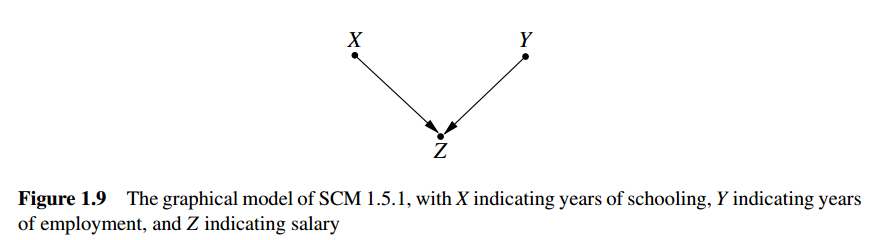
\includegraphics[scale = 0.5]{scm_graph.png}}
\end{minipage}
\caption{\footnotesize{\textbf{The graphical model representation of a structural causal model  \citep{pearl2009causal}}}}
\label{fig: scm_graph}
\end{figure}

\item Every SCM is associated with a \textbf{\emph{graphical causal model}}. Graphical models consist of a set of nodes representing the variables in $\mb{U}$ and $\mb{V}$, and a set of \emph{\textbf{edges}} between the nodes representing the functions in $\mb{F}$. 

\item We can define \textbf{causality} in terms of directed graphical models: If, in a graphical model, a variable $X$ is the \textbf{child} of another variable $Y$, then $Y$ is a \textbf{direct cause} of $X$; if $X$ is a \emph{\textbf{descendant}} of $Y$, then $Y$ is a \underline{\emph{\textbf{potential cause}}} of $X$. In this way, \textbf{the causal graphical model encodes the \emph{causal relationship assumptions}}. This is in contrast to the traditional directed graphical model, which encodes the \emph{associational relationship assumptions} such as conditional independence.
\end{itemize}

Figure \ref{fig: scm_graph} shows an example for SCM. This model represents the salary $Z$ that an employer pays an individual with $X$ years of
schooling and $Y$ years in the profession. $X$ and $Y$ both appear in $f_{Z}$, so $X$ and $Y$ are both direct causes of $Z$. If $X$ and $Y$ had any ancestors, those ancestors would be potential causes of $Z$.
\begin{align*}
\mb{U} = \{X, Y\}, \mb{V} = \{Z\},  \mb{F} = \{f_Z\} \\
f_Z: Z = 2X + 3Y
\end{align*}

\subsection{Structural Equations}
\begin{itemize}
\item In its general form, a \emph{\textbf{functional causal model}} consists of a set of equations of the form
\begin{align}
x_i &=  f_i (pa_i, u_i), \quad i = 1, \ldots, n, \label{eqn: structural_eqn}
\end{align}
where  \emph{parents} $pa_i$, stands for the set of variables that directly determine the value of $X_i$ and where the $U_i$ represent \emph{\textbf{errors}} (or \emph{\textbf{"disturbances"}}) due to omitted factors. Equation \eqref{eqn: structural_eqn} is a \emph{nonlinear}, \emph{nonparametric generalization} of the \emph{\textbf{linear structural equation models} (SEMs)}
\begin{align}
x_i &=  \sum_{k\neq 1}\alpha_{k,i} x_{k}   + u_i, \quad i = 1, \ldots, n, \label{eqn: linear_structural_eqn}
\end{align}
which have become a standard tool in economics and social science. In linear models, $pa_i$ corresponds to those variables on the r.h.s. of \eqref{eqn: linear_structural_eqn} that have nonzero coefficients. 

\item The function forms in \eqref{eqn: structural_eqn} can be \emph{laws} in physics and the natural sciences. They describe a set of \emph{\textbf{derterministic}} causal dependencies of $X_i$ to its parents and external factors $(PA_i, U_i)$. A set of equations in the form of  \eqref{eqn: structural_eqn} and in
which each equation represents an \emph{autonomous mechanism} is called a \emph{\textbf{structural model}}; if each variable has a distinct equation in which it appears on the left-hand side (called the \emph{dependent variable}), then the model is called a \underline{\emph{\textbf{structural causal model}}} (or, a causal model for short).

\item Note that compared to \textbf{potential outcome theory},
\begin{itemize}
\item the SCM views the intervention $do(x)$ as an \underline{\emph{\textbf{operation}}} that \underline{\textbf{changes the model}} (and the distribution) but keeps all variables the same;

\item the potential-outcome approach views the \textbf{outcome variable} $Y$ under $do(x)$ to be a \textbf{different variable}, $Y(x)$, loosely connected to $Y$ through relations such as \eqref{eqn: consistency}. 
\end{itemize}
\end{itemize}






\newpage
\section{Basic process in Causal Inference}
\begin{figure}
\begin{minipage}[t]{1\linewidth}
  \centering
  \centerline{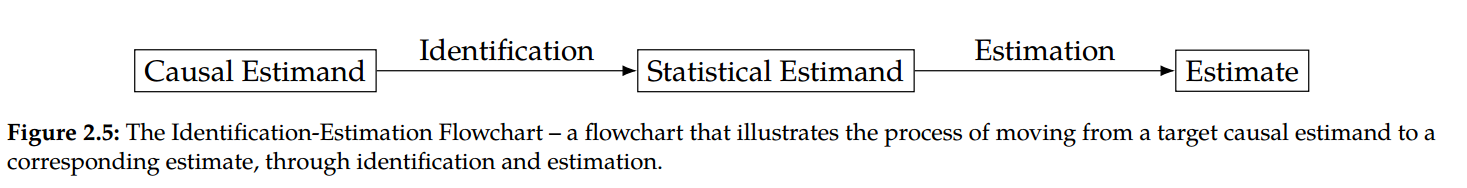
\includegraphics[scale = 0.35]{idt_est.png}}
\end{minipage}
\caption{\footnotesize{\textbf{The basic process of identification and estimation in causal inference.  \citep{neal2020introduction}}}}
\label{fig: idt_est}
\end{figure}

From the Adjustment Formula \eqref{eqn: ATE_2}, we see that there is a process for causal inference: 
\begin{enumerate}
\item \textbf{\emph{Causal Identification}}. In this process, we move from a \emph{\textbf{causal estimand}} to an equivalent \emph{\textbf{statistical estimand}} under various causal assumptions (\emph{unconfoundedness, positivity, and consistency}). That is from $\E{}{Y(1) - Y(0) | X} \rightarrow  \E{X}{ \E{}{Y \,|T=1,\,X }} - \E{X}{\E{}{Y \,|T=0, \, X}}$

\item \textbf{\emph{Statistical Estimation}}. In this process, we move from a \emph{statistical estimand} to an \textbf{estimate}. That is to find an estimate of $\E{}{Y \,|T=t, \, X=x}$ using models or statistical methods.
\end{enumerate}

\begin{figure}
\begin{minipage}[t]{1\linewidth}
  \centering
  \centerline{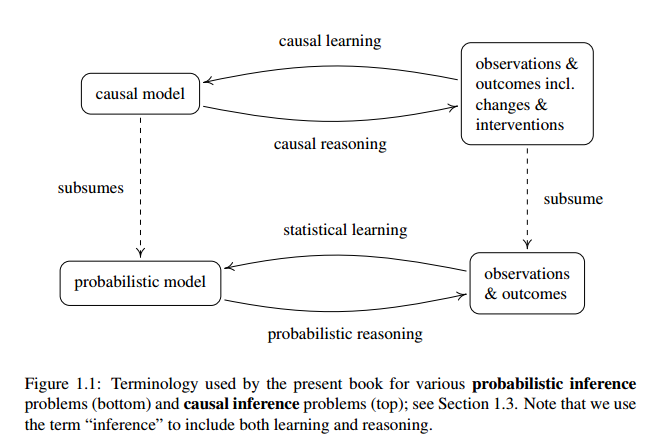
\includegraphics[scale = 0.6]{causal_learning.png}}
\end{minipage}
\caption{\footnotesize{\textbf{The probabilistic inference
problems (bottom) and causal inference problems.  \citep{peters2017elements}}}}
\label{fig: causal_learning}
\end{figure}

Figure \ref{fig: causal_learning} shows the relationships between statistical modeling and causal modeling \citep{peters2017elements}. Causal modeling starts from another, arguably more fundamental, structure. A causal structure \emph{\textbf{entails}} a probability model, but it contains additional information not contained in the latter.
\begin{itemize}
\item \textbf{\emph{Causal reasoning}}, according to the terminology used in \citep{peters2017elements}, denotes the process of drawing conclusions from a causal model, similar to the way probability theory allows us to reason about the outcomes of random experiments.


\item Just like statistical learning denotes the inverse problem to probability theory, \textbf{\emph{causal learning}} studies how to infer causal structures from its empirical implications.  The empirical implications can be purely observational, but they can also include data under interventions (e.g., randomized trials) or distribution changes. Researchers use various terms to refer to these problems, including \emph{\textbf{structure learning}} and \emph{\textbf{causal discovery}}.

\item \textbf{\emph{Structure identifiability}} is mainly concerned about the question of which parts of the \emph{\textbf{causal structure}} can in principle be inferred from the \emph{joint distribution}.

\item  \textbf{\emph{Causal learning}} is the \emph{inverse problem} of causal reasoning. Unlike the standard problems of statistical learning, \emph{even full knowledge of $P$ does not make the solution trivial}, and we need \textbf{additional assumptions} (see above). The diffculties in causal learning  not only include the  ill-posed-ness of the usual statistical problems, but also arise from the fact that we are trying to estimate a richer structure than just a probabilistic one.

\item It is less well known that one may postulate that while we cannot infer a concrete causal structure, we may at least \textbf{infer the existence} of causal links from statistical dependences. 
\begin{proposition}(\textbf{Reichenbach's common cause principle}) \citep{peters2017elements}\\
 If two random variables $X$ and $Y$ are \textbf{statistically dependent} ($X \not\indep Y$ ), then there exists a third variable $Z$ that \textbf{causally influences both}. (As a special case, $Z$ may coincide with either $X$ or $Y$.) Furthermore, this variable $Z$ screens $X$ and $Y$ from each other in the sense that given $Z$, they become independent,  $X \indep Y | Z$.
\end{proposition}
\end{itemize}

\newpage
\bibliographystyle{plainnat}
\bibliography{book_reference.bib}
\end{document}